\chapter{MacroRay Three-Dimensional Ray-tracing Technique}{\label{ch:MacroRay}
  %%% Multi-group Energy quantities %%%
\DeclareDocumentCommand{\gprime}{}{g^{\prime}}
% Cross-sections
\DeclareDocumentCommand{\xs}{ O{t} O{\loc} O{g}}{\ensuremath{\CrossSection_{#1}^{#3}(#2)}}
\DeclareDocumentCommand{\xst}{ O{\loc} O{g} }{\xs[t][#1][#2]}
\DeclareDocumentCommand{\xsa}{ O{\loc} O{g} }{\xs[a][#1][#2]}
\DeclareDocumentCommand{\xsf}{ O{\loc} O{\gprime} }{\xs[f][#1][#2]}
\DeclareDocumentCommand{\xss}{ o O{\loc} O{\dirprime\vdot\dir} O{\gprime \to g} }{
    \IfNoValueOrEmptyTF{#1}
    {\xs[s][#2,#3][#4]}
    {\xs[s,#1][#2][#4]}
}
\DeclareDocumentCommand{\spect}{ O{\loc} O{g} }{\ensuremath{\Spectrum^{#2}(#1)}}
\DeclareDocumentCommand{\nufis}{ O{\loc} O{\gprime} }{ \ensuremath{\nu\xsf[#1][#2]}}
\DeclareDocumentCommand{\D}{ O{\loc} O{g} }{\ensuremath{D^{#2}(#1)}}

% Flux
\DeclareDocumentCommand{\aflux}{ O{\loc} O{\dir} O{g} }{\ensuremath{\AngularFlux^{#3}(#1,#2)}}
\DeclareDocumentCommand{\sflux}{ O{\loc} O{\gprime} }{\ensuremath{\ScalarFlux^{#2}(#1)}}
\DeclareDocumentCommand{\current}{ O{\loc} O{g} }{\ensuremath{\Current^{#2}(#1)}}
\DeclareDocumentCommand{\fluxmoma}{ O{\ell} O{n} O{\loc} O{g} }{\ensuremath{\ScalarFlux^{#2,#4}_{#1}(#3)}}

% Source
\DeclareDocumentCommand{\source}{ O{\loc} O{\dir} O{g} }{\ensuremath{q^{#3}(#1,#2)}}
\DeclareDocumentCommand{\sourcemoma}{ O{\ell} O{n} O{\loc} O{g} }{\ensuremath{q^{#2,#4}_{#1}(#3)}}

  %%% Discrete Ordinates Quantities %%%
\DeclareDocumentCommand{\mprime}{}{m^{\prime}}
\DeclareDocumentCommand{\dirm}{ O{m} }{\dir_{#1}}
\DeclareDocumentCommand{\wt}{ O{m} }{\Weight_{#1}}

% Quadrature set
\DeclareDocumentCommand{\angquad}{ O{N} }{ \mathcal{M}_{#1} }

% Cross-Sections
\DeclareDocumentCommand{\xss}{ o O{\loc} O{ m^{\prime}\!\to m} O{\gprime\!\to g} }{
    \IfNoValueOrEmptyTF{#1}
    {\xs[s,#3][#2][#4]}
    {\xs[s,#1][#2][#4]}
}

% Flux
\DeclareDocumentCommand{\aflux}{ O{\loc} O{m} O{g}}{\ensuremath{\AngularFlux^{#3}_{#2}\!\left(#1\right)}}

% Source
\DeclareDocumentCommand{\source}{ O{\loc} O{m} O{g} }{\ensuremath{q^{#3}_{#2}\!\left(#1\right)}}

  %%% MOC quantities %%%
% Geometric
\DeclareDocumentCommand{\Length}{}{s}
\DeclareDocumentCommand{\NormalizedLength}{}{t}
\DeclareDocumentCommand{\len}{ O{} }{\Length_{#1}}
\DeclareDocumentCommand{\segl}{ O{mki} }{\Length_{#1}}
\DeclareDocumentCommand{\nlen}{ O{m} }{\NormalizedLength_{#1}}
\DeclareDocumentCommand{\nsegl}{ O{mki} }{\NormalizedLength_{#1}}

\DeclareDocumentCommand{\centroid}{ O{\loc} O{i} }{#1_{#2}^{\text{c}}}
\DeclareDocumentCommand{\locIn}{ O{\loc} O{mki} }{{#1}_{#2}^{\text{in}}}
\DeclareDocumentCommand{\locOut}{ O{\loc} O{mki} }{{#1}_{#2}^{\text{out}}}
\DeclareDocumentCommand{\locCent}{ O{\loc} O{mki} }{{#1}_{#2}^{\text{c}}}
\DeclareDocumentCommand{\M}{ o O{i}}{%
    \IfNoValueOrEmptyTF{#1}
        {\vec{M}_{#2}}
        {M_{#2,#1}}
}
\DeclareDocumentCommand{\C}{o O{i} O{g}}{%
    \IfNoValueOrEmptyTF{#1}
        {\vec{C}_{#2}^{#3}}
        {C_{#2,#1}^{#3}}
}


% Integration
\DeclareAutoPairedDelimiter{\MOCTrackIntegral}{\langle}{\rangle_{mki}}
\DeclareAutoPairedDelimiter{\MOCSingleAngleIntegral}{\langle}{\rangle_{mi}}
\DeclareAutoPairedDelimiter{\MOCIntegral}{\langle}{\rangle_{i}}

% Cross-sections
\DeclareDocumentCommand{\xs}{ O{t} O{i} O{g}}{\ensuremath{\CrossSection_{#1,#2}^{#3}}}
\DeclareDocumentCommand{\xst}{ O{i} O{g} }{\xs[t][#1][#2]}
\DeclareDocumentCommand{\xsa}{ O{i} O{g} }{\xs[a][#1][#2]}
\DeclareDocumentCommand{\xsf}{ O{i} O{\gprime} }{\xs[f][#1][#2]}
\DeclareDocumentCommand{\xss}{ o O{i} O{m'\to m} O{\gprime \to g} }{
    \IfNoValueOrEmptyTF{#1}
    {\xs[s][#2,#3][#4]}
    {\xs[s,#1][#2][#4]}
}

\DeclareDocumentCommand{\spect}{ O{i} O{g} }{\ensuremath{\Spectrum^{#2}_{#1}}}
\DeclareDocumentCommand{\nufis}{ O{i} O{\gprime} }{ \ensuremath{\nu\xsf[#1][#2]}}
\DeclareDocumentCommand{\D}{ O{i} O{g} }{\ensuremath{D^{#2}_{#1}}}
\DeclareDocumentCommand{\opt}{ O{m} O{g} }{\OpticalThickness_{#1}^{#2}}
\DeclareDocumentCommand{\segopt}{ O{mki} O{g} }{\opt[#1][#2]}

% MOC Parameters
\DeclareDocumentCommand{\tA}{ O{a} }{\ensuremath{\delta\!A_{#1}}}
\DeclareDocumentCommand{\Weight}{}{w}
\DeclareDocumentCommand{\wt}{ O{m} }{\Weight_{#1}}
\DeclareDocumentCommand{\wtbar}{ O{m} }{\overline{\Weight}_{#1}}
\DeclareDocumentCommand{\renorm}{ O{i} }{\ensuremath{\xi_{#1}}}

% Flux
\DeclareDocumentCommand{\aflux}{ O{mki} O{g} O{\len} }{
    \IfNoValueOrEmptyTF{#3}
    {\AngularFlux^{#2}_{#1}}
    {\ensuremath{\AngularFlux^{#2}_{#1}\!\left(#3\right)}}
}
\DeclareDocumentCommand{\afluxin}{ O{mki} O{g} }{\AngularFlux^{#2,\text{in}}_{#1}}
\DeclareDocumentCommand{\afluxout}{ O{mki} O{g} }{\AngularFlux^{#2,\text{out}}_{#1}}
\DeclareDocumentCommand{\sflux}{ O{g} O{i} }{\ScalarFlux_{#2}^{#1}}
\DeclareDocumentCommand{\current}{ O{i} O{g} }{\Current^{#2}_{#1}}
\DeclareDocumentCommand{\tfluxF}{ O{mki} O{g} }{ \overline{\AngularFlux}_{#1}^{#2} }          % Average flux-moment along track
\DeclareDocumentCommand{\tfluxL}{ O{mki} O{g} }{  \widehat{\AngularFlux}_{#1}^{#2} }          % Linear flux-moment along track
\DeclareDocumentCommand{\dflux}{ O{mki} O{g} }{ \Delta\AngularFlux_{#1}^{#2} }                % Difference of angular flux along track
\DeclareDocumentCommand{\sfluxF}{ O{i} O{g} }{ \overline{\ScalarFlux}_{#1}^{#2} }             % Average scalar flux
% \DeclareDocumentCommand{\sfluxL}{ o O{i} O{g} }{ % Linear expansion coeff (Scalar Flux)
%     \IfNoValueOrEmptyTF{#1}
%         {\lvec{\widehat{\ScalarFlux}}_{#2}^{#3}}
%         {\widehat{\ScalarFlux}_{#2,#1}^{#3}}
% }
\DeclareDocumentCommand{\sfluxL}{ O{i} O{g} o }{ % Linear expansion coeff (Scalar Flux)
    \IfNoValueOrEmptyTF{#3}
        {\lvec{\widehat{\ScalarFlux}}_{#1}^{#2}}
        {\widehat{\ScalarFlux}_{#1,#3}^{#2}}
}
% \DeclareDocumentCommand{\sfluxL}{ m O{i} O{g} }{\widehat{\ScalarFlux}_{#2,#1}^{#3} }          % Linear expansion coeff (Scalar flux)
\DeclareDocumentCommand{\afluxmom}{ O{\ell} O{n} O{i} O{\gprime} }{\FluxMoment_{#3,#1}^{#4,#2}}

% Source
\DeclareDocumentCommand{\source}{ O{mki} O{g} O{\len} }{\ensuremath{q^{#2}_{#1}\!\left(#3\right)}}
\DeclareDocumentCommand{\tsrcF}{ O{mki} O{g} }{ \overline{q}_{#1}^{#2} }          % Average source along track
\DeclareDocumentCommand{\tsrcL}{ O{mi} O{g} }{ \widehat{q}_{#1}^{#2} }          % Linear source along track
\DeclareDocumentCommand{\src}{ O{i} O{g} }{ \Source_{#1}^{#2}}                          % Generic source
\DeclareDocumentCommand{\srcF}{ O{i} O{g} }{ q_{#1}^{#2} }             % Average source
\DeclareDocumentCommand{\srcL}{ o O{i} O{g} }{ % Linear expansion coeff (Source)
    \IfNoValueOrEmptyTF{#1}
        {\lvec{\widehat{q}}_{#2}^{#3}}
        {\widehat{q}_{#2,#1}^{#3}}
}

% Linear source operators / functions
\DeclareDocumentCommand{\FluxToSource}{ O{g} }{\mathcal{S}^{#1}}
  \def\figpath{chapters/MacroRay/figures/}
  \graphicspath{ {\figpath} }

  The primary motivation of the three-dimensional macroray ray-tracing technique is to reduce the number of tracks generated for 3-D \ac{MOC} applications.
  The number of track-segments is very strongly correlated with the run-time of a \ac{MOC} calculation \footnote{if the \ac{MOC} calculation performs an entirely separate calculation (i.e does not use the chord-classification method) for each track-segment, this is expected to be directly proportional (ignoring overhead)}.
  The 2-D macroband ray-tracing method had been shown to allow for coarser ray-spacing compared to traditional methods, but has never been extended for use in 3-D \ac{MOC} calculations.
  This work seeks to fill that gap, and perform an investigation into the extension from 2-D to 3-D macroband-like ray-tracing.
  The ray-tracing technique is referred to as the \emph{macroray}, because the 3-D ``macro''paths are no longer bands, but instead parallel-pipes.

  This work implemented a 3-D ray-tracing and transport solver library in MPACT based on the macroray method.
  The initial step in this implementation was to implement a 2-D version \footnote{which did not support \ac{CMFD}}.
  This also serves to confirm the results of previous studies on 2-D macroband \cite{Yamamoto2005,Fevotte2007}.
  % These results will be presented in \cref{sec:MacroRay:Results2D}, while 3-D results are presented in \cref{sec:macroRay:Results3D}.

  \section{MacroRay Technique}{\label{sec:MR:MacroRay Technique}
    The macroray ray-tracing technique is a 3-D extension of the macroband method; in order to describe this new ray-tracing technique it is first necessary to describe the macroband method.
    \Cref{ssec:RT:Macroband} gave a brief summary of the history of macroband, as well as some benefits of the method.
    This section will serve to describe the macroband method in more detail, and show how the method is extended to 3-D.

    \subsection{Macroband Technique}{\label{ssec:MR:Macroband Technique}
      The macroband was first used in the \acf{CP} code HELIOS, and was considered to be essential for the stability of the method \cite{Villarino1992}.
      Unlike the traditional uniform/equidistant ray-tracing methods, the macroband method guarantees that each ray within a macroband will pass through the same regions, and not have any regions within its' bounds that are not crossed by the rays.
      This means that the placement of rays, and their widths, are determined by the internal geometry of the pin or subdomain that is being traced.
      Because there are no material discontinuities within a macroband, the track-segment average values are expected to be smooth in the transverse direction.
      This allows for the use of more advanced transverse integration, such as Gauss-Legendre quadrature integration \cite{Yamamoto2005}.

      The macroband method ray-tracing is described in \cref{alg:Macroband:Ray-tracing}.
      A downside of this method, is that each ray has a unique width which requires additional storage.
      However, all rays within a macroband pass through the same segments, so the region index for each segment only needs to be stored once, reducing memory by a larger amount.
      The process is shown visually in \cref{fig:MR:Macroband Process}.

      \begin{algorithm}[ht]
        \centering
        \caption{Macroband ray-tracing procedure for a pin-cell.\label{alg:Macroband:Ray-tracing}}
        \begin{algorithmic}[1]
          \State{Begin with a pin-cell geometry/mesh, and a direction of flight $\dirm$.}
          \State{Create a list of points, $P$, containing:
            \begin{enumerate}
              \item{corners,}
              \item{mesh intersections,}
              \item{and tangent points.}
            \end{enumerate}
          }
          \State{Sort the points by signed distance in normal direction, $\widehat{n}_m$, from center of pin}
          \State{The macrobands are bounded in the transverse direction by these distances}
          \ForAll{Macrobands}
            \State{Determine quadrature points and widths in transverse direction}
            \State{Place rays at these points with these widths}
            \State{Trace each ray}
          \EndFor
        \end{algorithmic}
      \end{algorithm}

      \begin{figure}[ht]
        \centering
        \begin{subfigure}[t]{0.33\linewidth}
          \centering
          \def\svgwidth{0.95\linewidth}
          \input{\figpath/Macroband/MacroBandProcess1.pdf_tex}
          \caption{Determine intersection and tangent points}
        \end{subfigure}%
        \hfill
        \begin{subfigure}[t]{0.33\linewidth}
          \centering
          \def\svgwidth{0.95\linewidth}
          \input{\figpath/Macroband/MacroBandProcess2.pdf_tex}
          \caption{Determine macroband boundaries (through identified points)}
        \end{subfigure}%
        \hfill
        \begin{subfigure}[t]{0.33\linewidth}
          \centering
          \def\svgwidth{0.95\linewidth}
          \input{\figpath/Macroband/MacroBandProcess3.pdf_tex}
          \caption{Perform ray-tracing within macroband boundaries}
        \end{subfigure}
        \caption{Ray-tracing process for macroband.}
        \label{fig:MR:Macroband Process}
      \end{figure}
    }
    There have been different approaches to 3-D ray-tracing for \ac{MOC}; the most common approach is to first generate 2-D tracking data, forming characteristic planes.
    Then 2-D tracking data is generated for each of the characteristic planes.
    This process was described in detail in \cref{ssec:RT:Three-Dimensional Ray-Tracing Techniques}, and will be referred to as the 2D/2D ray-tracing approach.
    This was the approach taken for this thesis work, but other approaches may have significant advantages; these will be discussed in \cref{ssec:MR:Interface Angular Flux Approximation}.

    Although previous works have investigated the 2-D macroband ray-tracing method \cite{Yamamoto2005,Fevotte2007,Yamamoto2008}, there have not been any studies in the extension of macroband to 3-D \ac{MOC} calculations.
    Here, the macroray ray-tracing technique uses the macroband method for both the 2-D radial track generation, and 2-D track generation within each characteristic plane.
    The setup procedure of the macrorays guarantee that their rays pass through the same regions, just as the macroband's did.
    However, it is no longer guaranteed that any region which is contained within the volume of a macroband will be passed through.
    This leads to some issues which will be discussed in \cref{ssec:MR:Interface Angular Flux Approximation}.

    Similarly to the macroband method, the macroray method is fundamentally incompatible with the \ac{DNPL} ray-tracing technique.
    The \ac{MRMB} technique can be used to store tracking data for unique geometric subsystems (typically a pin cell), greatly reducing
    Although tracking data can be generated for unique geometry subsystems (\ac{MRMB} \cite{Yamamoto2005}), some approximation of the angular flux is necessary on interfaces.
    Generally, the macroray and macroband methods, which provide more accurate integration, exchange regional numerical dispersion for interface numerical dispersion \cite{Sanchez2012}.
    It is the point of view of the author, that this is generally considered a favorable trade-off, as the engineering quantities of interest are primarily determined through regional integration.

    \subsection{Chord-Classification}{\label{ssec:MR:Chord-Classification}
      The chord-classification ray-tracing method \cite{Sciannandrone2016} was described in detail in \cref{sssec:RT:Chord-Classification}.
      One of the key criticisms of this method, by \citet{Gunow2018}, was that full 3-D tracking data needed to be generated prior to the classification of rays.
      However, with the addition of the macroray ray-tracing method, classification can be done automatically.

      During the axial ray-tracing along a characteristic plane, the computational mesh is used to determine the axial macrobands.
      Each ray within the macroray is guaranteed to pass through the same regions and surfaces; this means that each ray within an axial macroband is guaranteed to be of the same chord classification.
      This is demonstrated visually in \cref{fig:RT:Chord-Classification Macroray}.
      The chord-classification drastically cuts down on the amount of memory used to store 3-D tracking data, and also may reduce the amount of computational work.
      The work is reduced because the exponential functions (see \cref{sec:LSMOC:Exponential Tabulation}) are determined by the material and segment length.
      For vertical-to-vertical or horizontal-to-horizontal macroray segments, the segment lengths of all rays are the same, thus only a single exponential calculation is necessary.

      The chord-classification approach was taken in this work, rather than on-the-fly ray-tracing \cite{Gunow2018}.
      This was done due to the ease of implementation (because of automatic classification), and because of the criticisms of on-the-fly ray-tracing described in \cref{ssec:RT:On-the-Fly Ray-Tracing}.

      \begin{figure}[h]
        \centering
        \def\svgwidth{0.45\linewidth}
        \input{\figpath/ChordClassificationMacroBand.pdf_tex}
        \caption{3-D example of chord-classification with Macroray ray-tracing. Colored (red and blue) characteristic tracks represent groups of ``V-chords'', rays between two vertical surfaces.}
        \label{fig:RT:Chord-Classification Macroray}
      \end{figure}
    }

    \subsection{Interface Angular Flux Approximation}{\label{ssec:MR:Interface Angular Flux Approximation}
      In \cref{sssec:RT:Interface Flux Approximations} different approaches to approximating the angular flux on the boundaries was outlined for a 2-D macroband-based \ac{MOC} calculation.
      A ``fraction contribution'' sub-boundary averaging technique was described and chosen as the approach for this work.
      In this approach, each surface of the subsystems (pin cells) is divided into sub-boundaries based on the direction of flight.
      Each ray's width is considered, and partial intersections with each surface are computed and used to determine the ray's fractional contribution to each sub-boundary.
      And in the reverse direction (going from sub-boundary to ray), each sub-boundaries fractional contribution to each ray is determined.
      It was shown that this method conserved the total area-integrated angular flux on each surface.

      However, in 3-D this approach becomes considerably more complicated due to the nature of 3-D geometries and the 2D/2D ray-tracing approach.
      This cause of the issues stems from the fact that each ray, as viewed in the direction of flight, is rectangular.
      Each ray is rectangular because in the radial ray-tracing step, the ray is considered within the bounds of the width in the radially transverse direction, and in the axial ray-tracing on the characteristic plane the ray is again constrained in a height in the axially transverse direction.
      The rectangular ray projection is demonstrated for a single ray in \cref{figs:MR:MacroRayProjections}.

      For 3-D extruded cartesian pin cells, it is impossible (in arbitrary directions) to ``span''\footnote{in this context, ``span'' will be used to describe the idea that each ray's entire area projects onto some surface, and the entire surface is filled with ray projections.} the surfaces of our system.
      Because each ray is rectangular, parts of the pin cell's surfaces will not be ``hit'' by the projection of any ray, and parts of some rays will live entirely outside the problem domain.
      This issue is visualized in \cref{fig:MR:MacroRayProjectionProblem}; it should also be noted that the area outside the domain, and the surface area without any covering rays are not equal in area unless the ray is in the center of the radial width.

      \begin{figure}[htbp]
          \centering
          \begin{subfigure}[t]{0.45\textwidth}
              \centering
              \def\svgwidth{0.70\linewidth}
              \input{\figpath/MacroRayProjections.pdf_tex}
              \caption{2-D ray viewed from above\label{fig:MR:MacroRayProjections}}
          \end{subfigure}%
          \begin{subfigure}[t]{0.45\textwidth}
              \centering
              \def\svgwidth{0.70\linewidth}
              \input{\figpath/MacroRayProjectionsDOF.pdf_tex}
              \caption{3-D ray viewed in direction of flight\label{fig:MR:MacroRayProjectionsDOF}}
          \end{subfigure}
          \caption{Example of the projected rectangular area formed in the 2D/2D ray-tracing approach.}
          \label{figs:MR:MacroRayProjections}
      \end{figure}

      \begin{figure}[htbp]
        \centering
        \def\svgwidth{0.25\linewidth}
        \input{\figpath/MacroRayProjectionsDOFProblem.pdf_tex}
        \caption{
            An example of a ray that causes issues with the fractional contribution interface flux approximation when using 2D/2D ray-tracing.
            The highlighted red area is the area of the ray outside the domain (which projects to no surface), and the blue highlighted area is an area on the surface that will not be hit by any ray.}
        \label{fig:MR:MacroRayProjectionProblem}
      \end{figure}

      The rays not ``spanning'' our system causes issues with the conservation of surface flux as described in \cref{sssec:RT:Interface Flux Approximations}.
      Previously, the average angular flux in a sub-boundary was determined by
      \begin{equation}\label{eq:MR:Old SubBoundary Flux}
        \psi_s^i = \suml[j] \frac{A(S_i\cap R_j)}{A(S_i)}\psi_r^j.
      \end{equation}
      It was shown that by summing over all sub-boundaries, the total flux passing through the surface was conserved.
      However, because the rays are no longer guaranteed to span the system's surfaces, the summation of intersected ray areas is no longer equal to the sub-boundary areas:
      \begin{equation}\label{eq:MR:Area Imbalance}
        \suml[j] A(S_i\cap R_j) \leq A(S_i).
      \end{equation}
      Generally, these areas are very close, and in the limit of infinite rays they are equivalent; but, the motivation of this work has been to reduce the number of rays, so this issue needs to be addressed.
      \Cref{sssec:MR:MacroRay Area Correction} describes how this issue was addressed in this work, and \cref{sssec:MR:Alternative Approaches} describes possible alternative approaches.

      \subsubsection{MacroRay Area Correction}{\label{sssec:MR:MacroRay Area Correction}
        Two ideas were investigated in order to address the issue of the rays not spanning the surface areas.
        Here, it should be emphasized that the first approach is \emph{incorrect}.
        It will be described in this section because it seems like a reasonable choice for this correction; in fact, it was not realized for some time in this work that the first approach was incorrect.

        The sub-boundary averaging method of this work has been referred to as a ``fractional contribution'' approach.
        This comes from \cref{eq:MR:Old SubBoundary Flux} where $A(S_i \cap R_j) / A(S_i)$ is the fractional contribution of flux from ray $j$ into sub-boundary $i$.
        In 2-D, these fractions will sum to one, because our rays span the surfaces of our system:
        \begin{equation}\label{eq:MR:2-D Fractional Unity}
          \suml[j] \frac{A(S_i \cap R_j)}{A(S_i)} = 1.
        \end{equation}

        The first approach taken attempted to preserve this property of fractional contributions summing to unity.
        This is done by ignoring ray areas outside the domain and surface areas that are not covered by ray projections; the sub-boundary and ray fluxes are determined by
        \begin{subequations}\label[subeqs]{eqs:MR:Flux A1}
          \begin{equation}\label{eq:MR:SubBoundary Flux A1}
            \psi_s^i = \suml[j] \frac{A(S_i \cap R_j)}{\suml[k] A(S_i \cap R_k)}\psi_r^j = \suml[j] \frac{A(S_i \cap R_j)}{A_p(S_i)}\psi_r^j,
          \end{equation}
          \begin{equation}\label{eq:MR:Ray Flux A1}
            \psi_r^j = \suml[i] \frac{A(S_i \cap R_j)}{\suml[k] A(S_k \cap R_j)}\psi_s^i = \suml[i] \frac{A(S_i \cap R_j)}{A_p(R_j)}\psi_s^i,
          \end{equation}
        \end{subequations}
        respectively.
        For convenience, let us define the ``total projected area'' as the sum of intersections for that object, for example the total projected area of a ray would be defined by
        \begin{equation}\label{eq:MR:Projected Area Ray}
          A_p(R_j) \defined \suml[i] A(S_i \cap R_j),
        \end{equation}
        and similarly for $A_p(S_i)$.
        Through these definitions the new fractional contributions sum to unity:
        \begin{subequations}\label[subeqs]{eqs:MR:Fractions A1}
          \begin{equation}\label{eq:MR:SubBoundary Fractions A1}
            \suml[j] \frac{A(S_i \cap R_j)}{A_p(S_i)} = 1,
          \end{equation}
          and
          \begin{equation}\label{eq:MR:Ray Fractions A1}
            \suml[i] \frac{A(S_i \cap R_j)}{A_p(R_j)} = 1.
          \end{equation}
        \end{subequations}

        While this may seem reasonable \footnote{at least at first to the author}, this is not actually the property we need to preserve for compatibility with \ac{CMFD} acceleration.
        The surface-integrated angular flux needs to be preserved, but in this first approach this is not the case.
        \begin{subequations}\label[subeqs]{eqs:MR:Flux Conservation A1}
          \begin{equation}\label{eq:MR:SubBoundary Flux Conservation A1}
            \psi_t^s = \suml[i] A(S_i) \psi_s^i
                     = \suml[i] A(S_i) \suml[j] \frac{A(S_i \cap R_j)}{A_p(S_i)}\psi_r^j
                     \neq \psi_t^r,
          \end{equation}
          \begin{equation}\label{eq:MR:Ray Flux Conservation A1}
            \psi_t^r = \suml[j] A(R_j) \psi_r^j
                     = \suml[j] A(R_j) \suml[i] \frac{A(S_i \cap R_j)}{A_p(R_j)}\psi_s^i.
                     \neq \psi_t^s,
          \end{equation}
        \end{subequations}
        Note that the true areas $A(S_i)$ and $A(R_j)$ must be used to sum the fluxes in order to integrate over the entire surface (or ray areas).

        This approach actually works for many problems, and while small differences between the solutions of transport and accelerated transport calculations, they are usually small.
        However, for larger problems, the \ac{CMFD} acceleration \emph{may} become unstable and cause the iteration scheme to diverge; though this generally only occurs if the convergence criteria is relatively low ($\leq 10^{-6}$).
        Nevertheless, compatibility with \ac{CMFD} acceleration, or other acceleration methods, is necessary if this method is ever to be used.
        This leads to the approach used for the remained of this work.

        As this section has emphasized, the property that is important to conserve is the surface-integrated angular flux.
        The surface-integrated angular flux can be found by integrating over sub-boundaries, or over rays; it is necessary for these to be equal:
        \begin{equation}\label{eq:MR:Surface-Integrated Angular Flux}
          \psi_t = \suml[i] A(S_i) \psi_s^i = \suml[j] A(R_j) \psi_r^j.
        \end{equation}
        The sub-boundary flux, $\psi_s^i$, should be dependent on the ray fluxes, $\psi_r^j$, and should also follow a similar form as \cref{eq:MR:Old SubBoundary Flux}.

        Let us examine the sub-boundary flux in order to show how the surface-integrated angular flux may be preserved.
        Insert a corrective multiplicative term into the summation of \cref{eq:MR:Old SubBoundary Flux},
        \begin{equation}\label{eq:MR:SubBoundary Flux:Derivation 1}
          \psi_s^i = \suml[j] k_s^{j} \frac{A(S_i \cap R_j)}{A(S_i)} \psi_r^j.
        \end{equation}
        Substituting this form into \cref{eq:MR:Surface-Integrated Angular Flux} yields,
        \begin{equation}\label{eq:MR:Surface-Integrated Angular Flux:Derivation 2}
          \psi_t = \suml[i] A(S_i) \suml[j] k_s^{j} \frac{A(S_i \cap R_j)}{A(S_i)} \psi_r^j = \suml[j] A(R_j) \psi_r^j.
        \end{equation}
        So, $k_s^{j}$ should be chosen such that
        \begin{equation}\label{eq:MR:ks factor condition}
          \suml[i] k_s^{j} A(S_i \cap R_j) = A(R_j),
        \end{equation}
        solved by
        \begin{equation}\label{eq:MR:ks factor}
          k_s^{j} = \frac{A(R_j)}{\suml[i] A(S_i \cap R_j)} = \frac{A(R_j)}{A_p(R_j)}.
        \end{equation}
        The sub-boundary flux can then be determined by
        \begin{subequations}\label[subeqs]{eqs:MR:Flux}
          \begin{equation}\label{eq:MR:SubBoundary Flux}
            \psi_s^i = \suml[j] \frac{A(R_j)}{A_p(R_j)}\frac{A(S_i \cap R_j)}{A(S_i)}\psi_r^j,
          \end{equation}
          and similarly, the ray flux can be determined by
          \begin{equation}\label{eq:MR:Ray Flux}
            \psi_r^j = \suml[i] \frac{A(S_i)}{A_p(S_i)}\frac{A(S_i \cap R_j)}{A(R_j)}\psi_s^i.
          \end{equation}
        \end{subequations}
        As this was derived from \cref{eq:MR:Surface-Integrated Angular Flux}, these forms guarantee that the surface-integrated angular flux is conserved.
        It should also be noted that if the surfaces are spanned by the rays the factors, $A(R_j)/A_p(R_j)$ and $A(S_i)/A_p(S_i)$, are one, giving back the original form of the equations.
      }

      \subsubsection{Alternative Approaches}{\label{sssec:MR:Alternative Approaches}
        The approach described in \cref{sssec:MR:MacroRay Area Correction} provided a correction to \cref{eq:MR:Old SubBoundary Flux} such that the surface-integrated angular flux is conserved.
        This approach seems to be valid when operating in the 2D/2D (rectangular) ray-tracing procedure, but there are alternative options.
        The reason a correction was necessary is because due to the nature of 3-D geometry and 2D/2D ray-tracing, the ray are no longer guaranteed to span the system's surfaces.
        It is possible to have an alternative ray-tracing approach (still based on the macroray) which does span the system's surfaces.

        The choice of rectangular rays was arbitrary, but this choice may be exchanged for any shape, such as triangular, or even arbitrarily shaped rays.
        Non-rectangular rays were not investigated as part of this work, and to the best of our knowledge, have not been investigated by any works.
        As previously mentioned, 3-D \ac{MOC} codes up to this point have used the uniform ray-spacing assumption in order to comply with constraints of \ac{MRT} and \ac{DNPL}.
        When rays are uniformly spaced and have \ac{DNPL}, the shape of the ray is largely ignored because the procedures only care about the ray's centroid.
        It only becomes important when you consider the integration volume of the ray, such as in the sub-boundary averaging method with fractional contributions.

        If rays are constructed so that they span the system's surfaces, there is no need to correct \cref{eq:MR:Old SubBoundary Flux}.
        It is not clear at this point whether or not this would have benefits for the accuracy of the method.
        However, it is possible to also preserves some of the desirable features for general geometries of the macroband which were lost in the transition to 3-D (in the 2D/2D ray-tracing framework).
        If the geometry is not locally extruded (in this work this was an assumption), then it is possible for macrorays to have some of their transverse area in a region that none of its' rays pass through.
        Examples of how non-rectangular rays might be used are shown in \cref{figs:MR:Alternatives}.

        \begin{figure}[h]
          \centering
          \begin{subfigure}[t]{0.32\textwidth}
            \centering
            \def\svgwidth{0.85\linewidth}
            \input{\figpath/MacroRayProjectionsGeom.pdf_tex}
            \caption{geometry\label{fig:MR:Alternatives:Geom}}
          \end{subfigure}%
          \begin{subfigure}[t]{0.32\textwidth}
            \centering
            \def\svgwidth{0.85\linewidth}
            \input{\figpath/MacroRayProjectionsDOFAlternative.pdf_tex}
            \caption{Axially stacked rays\label{fig:MR:Alternative 1}}
          \end{subfigure}%
          \begin{subfigure}[t]{0.32\textwidth}
            \centering
            \def\svgwidth{0.85\linewidth}
            \input{\figpath/MacroRayProjectionsDOFAlternative2.pdf_tex}
            \caption{General triangular rays\label{fig:MR:Alternative 2}}
          \end{subfigure}
          \caption{
            Two alternative (non-rectangular) ray-tracing ideas.
            (a) shows the geometry for clarity.
            (b) shows an example of rays which are generated to be axially aligned in a characteristic plane, but consider the full volume they pass through.
            (c) shows an example of triangulated rays.
            In both (b) and (c) the rays are formed by rhombuses or triangles, but if there were a cylinder in this pin, it is possible they could have curved boundaries as well.
          }
          \label{figs:MR:Alternatives}
        \end{figure}
      }
    }
  }

  % \section{MacroMoC Transport Library}{\label{sec:MacroMOC Transport Library}
  %   This work involved the implementation of a transport library based on the macroband and macroray ray-tracing techniques.
  %   This library is a sub-package dependent on MPACT for geometry, data, and iteration; the library was responsible for performing the ray-tracing, storage of tracking data, and the transport sweep calculations.
  %   The library was first implemented (without \ac{CMFD} support) for 2-D transport calculations using the macroband method.
  %   The library was then extended for 3-D transport calculations using the macroray method, with chord-classification.

  %   The library does not support the full range of geometries supported by MPACT; in particular, the graph-based geometry used for \acp{BWR} \cite{MPACTBWR2017} is not supported.
  %   Additionally, the directional quadratures were assumed to be product quadratures.
  % }



  % \section{Results - 2-D}{\label{sec:MacroRay:Results2D}
  %   This section will present 2-D macroband calculation results, which will help to give an estimate of what may be expected in 3-D.
  %   Each of these calculations was run without \ac{CMFD} acceleration, and with a Tabuchi-Yamamoto quadrature \cite{TabuchiYamamotoQuad} 64 azimuthal and 4 polar angles over $\fourpi$.
  %   Additionally, each case is run with the \ac{LSMOC} formulation described in \cref{ch:Improved Linear Source Formulation for Multi-physics and 2D/1D Applications}.
  %   Previous results \cite{Yamamoto2005} have shown that the use of a Gauss-Legendre quadrature for placing the macroband rays has significant accuracy benefits compared to spacing them uniformly within each band.

  %   % \subsection{C5G7 Pin-Cell}{\label{ssec:MB:C5G7 Pin-Cell}
  %   %   A single \ac{UO2} C5G7 \cite{Smith2006} pin-cell was used as an initial starting point to test the macroband method implemented in this work.
  %   %   This problem is relatively simple, and it is not expected to see significant difference between macroband and \ac{MRT} in this case.
  %   %   However, it can be used to test the
  %   % }

  %   \subsection{VERA Problem 1E}{\label{ssec:MB:VERA Problem 1E}
  %     VERA progression problem 1E \cite{VERAProblems} is a single \ac{IFBA} pin with a very thin coating of strong absorber.
  %     This case was selected for a 2-D study, as the previous \ac{LSMOC} results indicated that such pins, when in a lattice, prevented the use of coarse ray-spacing in the lattice calculations.
  %     If the macroband method can reduce the effective ray-spacing necessary for an accurate \ac{IFBA} pin calculation, this is a strong indication it will help in the lattice problems.
  %     Two different approaches were tested to determine the number of rays within a macroband: first, the width of the band is divided by the ray-spacing and the ceiling is taken.
  %     The second approach is to place a fixed number of rays within each band.

  %     \Cref{fig:MB:1e:keff-vs-rayspacing,fig:MB:1e:dk-vs-nSegs} show the eigenvalue results for a variety of effective ray-spacing, and the eigenvalue errors for the the number of ray-segments.
  %     Effective ray-spacing is computed by averaging the widths of all rays in the problem.
  %     In this case, the eigenvalue error is taken as the difference from the converged \ac{MRT} result.
  %     These figures show a clear advantages for the macroband ray-tracing method;
  %       even for the coarsest macroband spacing, the resulting eigenvalue was within 150 pcm of the converged result.
  %     The method using a fixed number of rays in each macroband seems to have an advantage when using coarse ray-spacings, and converges slightly faster than the width-determined number of rays per band.

  %     The convergence of the eigenvalue as more rays (segments) are added is very close to monotonic for the macroband methods.
  %     This is certainly not the case for the \ac{MRT} method, which sees very large swings in the eigenvalue from small changes in the ray-spacing, as shown by the large spikes in \cref{fig:MB:1e:pdk-vs-rayspacing}.
  %     The large spikes on the right of this plot show that for small changes in the ray-spacing, a large ($>2000$ pcm) reactivity swing can occur when using \ac{MRT}, whereas both macroband approaches have low differences between cases with similar ray-spacing.
  %     The lack of these large changes, allows the solver to act as more of a ``black box'', where the user does not need knowledge of the method to use it.
  %     Additionally, because of the near monotonic convergence behavior, it may be possible to use Richardson extrapolation to further reduce costs.

  %     \begin{figure}[htbp]
  %       \centering
  %       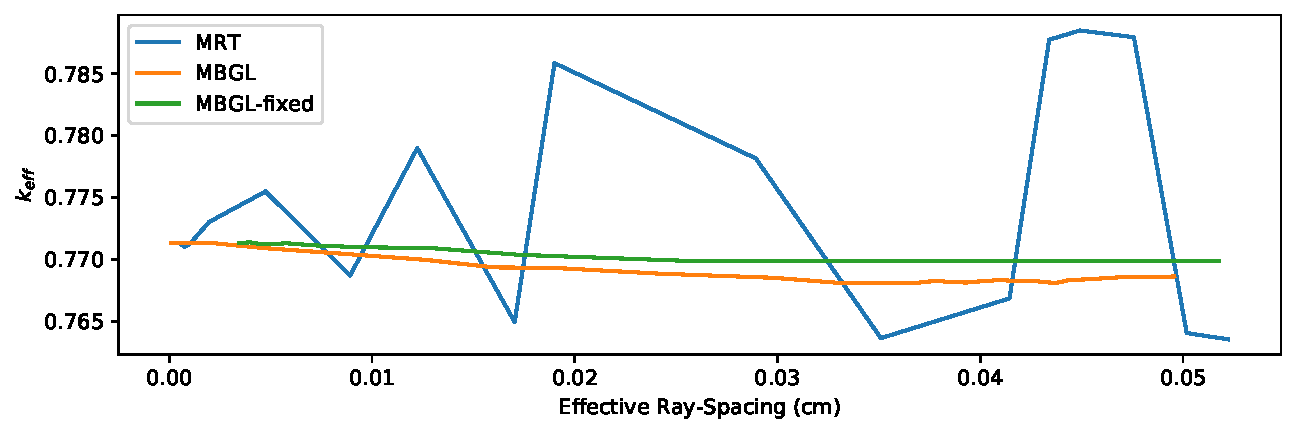
\includegraphics[width=0.95\linewidth]{\figpath/results/2D/1e/keff-vs-rayspacing}
  %       \caption{VERA Problem 1E: Eigenvalue results for different ray-tracing methods. \label{fig:MB:1e:keff-vs-rayspacing}}
  %     \end{figure}
  %     \begin{figure}[htbp]
  %       \centering
  %       \includegraphics[width=0.95\linewidth]{\figpath/results/2D/1e/dk-vs-nSegs}
  %       \caption{VERA Problem 1E: Eigenvalue errors for different ray-tracing methods. \label{fig:MB:1e:dk-vs-nSegs}}
  %     \end{figure}
  %     \begin{figure}[htbp]
  %       \centering
  %       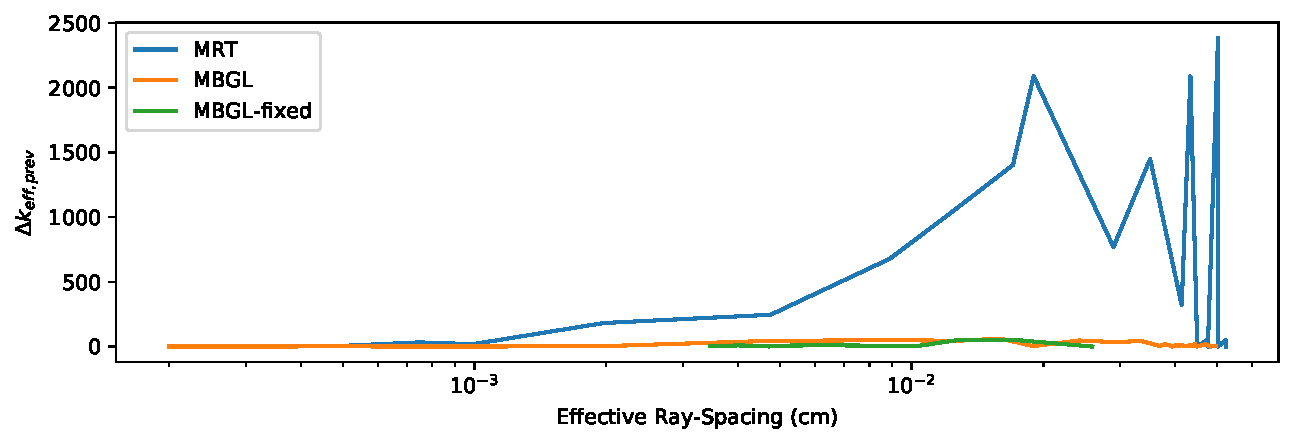
\includegraphics[width=0.95\linewidth]{\figpath/results/2D/1e/pdk-vs-rayspacing}
  %       \caption{VERA Problem 1E: Convergence of eigenvalue for different ray-tracing methods. \label{fig:MB:1e:pdk-vs-rayspacing}}
  %     \end{figure}
  %   }

  %   \subsection{VERA Problem 2}{\label{ssec:MB:VERA Problem 2}
  %     In \cref{ch:Improved Linear Source Formulation for Multi-physics and 2D/1D Applications}, the \ac{VERA} problem 2 lattices were tested with the improve \ac{LSA} formulation.
  %     One hypothesis going in, was that the use of the coarser mesh may allow for the use of coarser rays, thus much less work.
  %     However, it was found that the presence of any element with fine material discontinuities, such as control rods, or \acf{IFBA} rods, prevented the use of coarser rays while maintaining accuracy.
  %     In \cref{ssec:MB:VERA Problem 1E}, the macroband method was shown to be very advantageous compared to \ac{MRT} for a single \ac{IFBA} rod.
  %     In this section, the macroband method will be tested on two lattices from the \ac{VERA} problem 2 series that contain \ac{IFBA} rods: M, and N.

  %     [Paste results]

  %     % Two of the lattices, that presented issues for coarse ray spacing in \cref{ch:Improved Linear Source Formulation for Multi-physics and 2D/1D Applications}, were selected for study with the macroband: M and N.
  %     % Each of these cases has several \ac{IFBA} pins within the lattice, which require finer ray-spacing for accurate results.
  %   }
  % }

  % \section{Results}{\label{sec:MacroRay:Results3D}
  %   \subsection{C5G7 Pin-Cell}{\label{ssec:MR:C5G7 Pin-Cell}
  %     In this section, the results of 3-D \ac{MOC} calculations using the macroray ray-tracing method will be presented for a C5G7 \ac{UO2} pin-cell with different boundary conditions.
  %     A Chebyshev-Gauss product quadrature was used in each calculation, but the different boundary conditions will require different orders.
  %     For each case, a reference solution was generated using the openMC Monte Carlo code \cite{OpenMC}.
  %     The reference solution was generated with 500 batches of 50000 particles, with 50 inactive batches.
  %     2-D results have demonstrated that advantage of using fixed number of rays per macroband, thus a similar approach will be taken in these calculations.

  %     \subsubsection{Reflective}{\label{sssec:MR:C5G7:Pin:Reflective}
  %       First, a 1 cm tall pin-cell with reflective boundary conditions on all sides was used to verify that the 3-D macroray methods were generating correct results.
  %       This problem is equivalent to a 2-D transport problem, but for these calculations it will be solved using 3-D \ac{MOC}.
  %       This case used 16 azimuthal angles and varying numbers of polar angles from one to six.



  %     }

  %     \subsubsection{Vacuum-Top}{\label{sssec:MR:C5G7:Pin:Vacuum-Top}
  %       The same pin-cell was then run using similar conditions but with a vacuum boundary condition on the top surface.
  %       This case is meant to demonstrate that the macroray method is able to correctly handle an actual 3-D \ac{MOC} calculation.
  %     }
  %   }

  %   \subsection{VERA Problem 1E}{\label{ssec:MR:VERA Problem 1E}
  %     \ac{VERA} progression problem 1E is a relatively challenging pin-cell problem for transport methods due to the thin coating of boron on the fuel rod.
  %     This problem demonstrated clear advantages for the 2-D macroband method; in this section the problem is used to demonstrate the same for the 3-D macroray method.

  %     \subsubsection{Reflective}{\label{sssec:MR:1E:Reflective}

  %     }

  %     \subsubsection{Vacuum-Top}{\label{sssec:MR:1E:Vacuum-Top}

  %     }
  %   }

  %   \subsection{Shielded Fuel-Box}{\label{ssec:MR:Shielded Fuel-Box}
  %     The shielded fuel-box problem was created for this work to more clearly demonstrate the benefits of the macroray method for more general problems.
  %     This problem consists of a 0.4$\times$0.4$\times$0.4 cm$^3$ fuel block surrounded on all sides by $0.1$ cm of a shielding material.
  %     This entire shielded cube is surrounded by 0.5$\times$0.5$\times$0.5 cm$^3$ cubes of moderator (26 in total).
  %     The calculation uses the C5G7 benchmark cross sections; the fuel is the 8.7\% \ac{MOX}, the shielding material uses the control rod cross sections.
  %     A 2-D cross-sectional view of the problem is shown in [REF].

  %     [PICTURE OF PROBLEM].

  %   }
  % }

  \section{Results}{\label{sec:MR:Results}
    This section will present results using the macroray ray-tracing method, and comparing it against the \acf{MRT} method.
    All results presented use the \ac{LSA} approximation developed in \cref{ch:Improved Linear Source Formulation for Multi-physics and 2D/1D Applications}.

    \subsection{VERA Problem 1E}{\label{ssec:MR:VERA Problem 1E}
        % VERA progression problem 1E \cite{VERAProblems} is a single \ac{IFBA} pin with a very thin coating of strong absorber.
        % This case was selected for a 2-D study, as the previous \ac{LSMOC} results indicated that such pins, when in a lattice, prevented the use of coarse ray-spacing in the lattice calculations.
        % If the macroband method can reduce the effective ray-spacing necessary for an accurate \ac{IFBA} pin calculation, this is a strong indication it will help in the lattice problems.
        % Two different approaches were tested to determine the number of rays within a macroband: first, the width of the band is divided by the ray-spacing and the ceiling is taken.
        % The second approach is to place a fixed number of rays within each band.

      \ac{VERA} progression problem 1E \cite{VERAProblems} is a single \ac{IFBA} pin with a very thin coating of boron on the fuel.
      The boron will shield the pin from incident thermal neutrons, significantly dampening the reactivity.
      These rods are used in reactor designs, and as the fuel cycle continues the boron will be depleted and the reactivity will increase.

      Such a thin coating which has a very significant impact on the reactivity can be a difficult problem for transport methods.
      The \ac{MOC} is able to handle this case, but generally requires very fine ray-spacing in order to resolve these thin coating regions.
      This makes \ac{VERA} problem 1E a perfect test case for the macroband and macroray methods, which will automatically place rays through these thin regions.
      Ideally, this would allow coarser ray-spacing to be used elsewhere in the pin.

      \subsubsection{VERA Problem 1E: 2-D}{\label{sssec:MR:1E:2-D}
        Each calculation in this section used a Tabuchi-Yamamoto \cite{TabuchiYamamotoQuad} directional quadrature with 64 azimuthal angles and 4 polar angles over $\fourpi$.
        Additionally, a self-shielding calculation was run to compute macroscopic cross sections for the problem.
        Two different approaches were tested to determine the number of rays within a macroband: first, the width of the band is divided by the ray-spacing and the ceiling is taken.
        The second approach is to place a fixed number of rays within each band.

        \Cref{fig:MB:1e:keff-vs-rayspacing,fig:MB:1e:dk-vs-nSegs} show the eigenvalue results for a variety of effective ray-spacing, and the eigenvalue errors for the the number of ray-segments.
        Effective ray-spacing is computed by averaging the widths of all rays in the problem.
        In this case, the eigenvalue error is taken as the difference from the converged \ac{MRT} result.
        These figures show a clear advantages for the macroband ray-tracing method;
          even for the coarsest macroband spacing, the resulting eigenvalue was within 150 pcm of the converged result.
        The method using a fixed number of rays in each macroband seems to have an advantage when using coarse ray-spacings, and converges slightly faster than the width-determined number of rays per band.

        The convergence of the eigenvalue as more rays (segments) are added is very close to monotonic for the macroband methods.
        This is certainly not the case for the \ac{MRT} method, which sees very large swings in the eigenvalue from small changes in the ray-spacing, as shown by the large spikes in \cref{fig:MB:1e:pdk-vs-rayspacing}.
        The large spikes on the right of this plot show that for small changes in the ray-spacing, a large ($>2000$ pcm) reactivity swing can occur when using \ac{MRT}, whereas both macroband approaches have low differences between cases with similar ray-spacing.
        The lack of these large changes, allows the solver to act as more of a ``black box'', where the user does not need knowledge of the method to use it.
        Additionally, because of the near monotonic convergence behavior, it may be possible to use Richardson extrapolation to further reduce costs.

        \begin{figure}[hp]
          \centering
          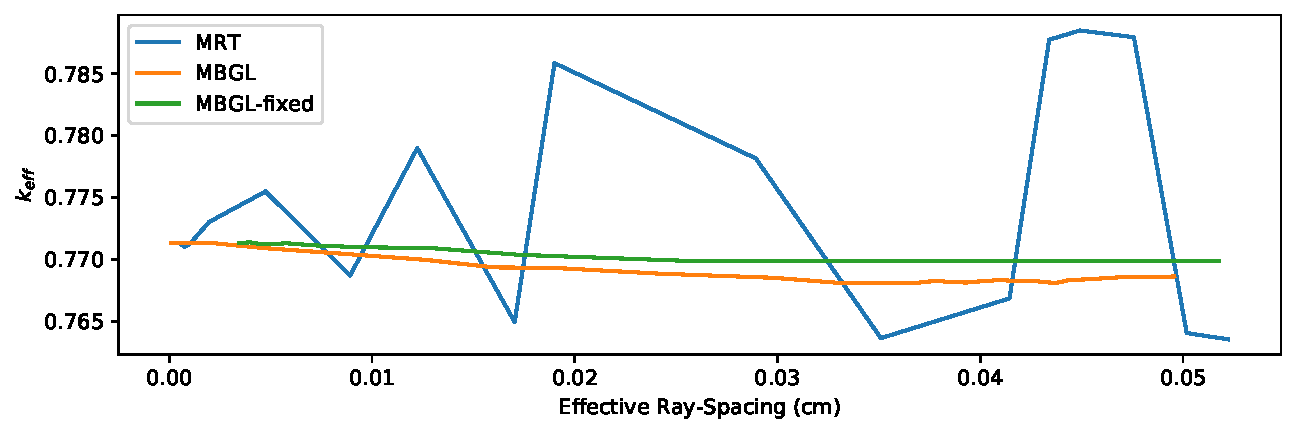
\includegraphics[width=0.95\linewidth]{\figpath/results/2D/1e/keff-vs-rayspacing}
          \caption{VERA Problem 1E: Eigenvalue results for different 2-D ray-tracing methods. \label{fig:MB:1e:keff-vs-rayspacing}}
        \end{figure}
        \begin{figure}[hp]
          \centering
          \includegraphics[width=0.95\linewidth]{\figpath/results/2D/1e/dk-vs-nSegs}
          \caption{VERA Problem 1E: Eigenvalue errors for different 2-D ray-tracing methods. \label{fig:MB:1e:dk-vs-nSegs}}
        \end{figure}
        \begin{figure}[hp]
          \centering
          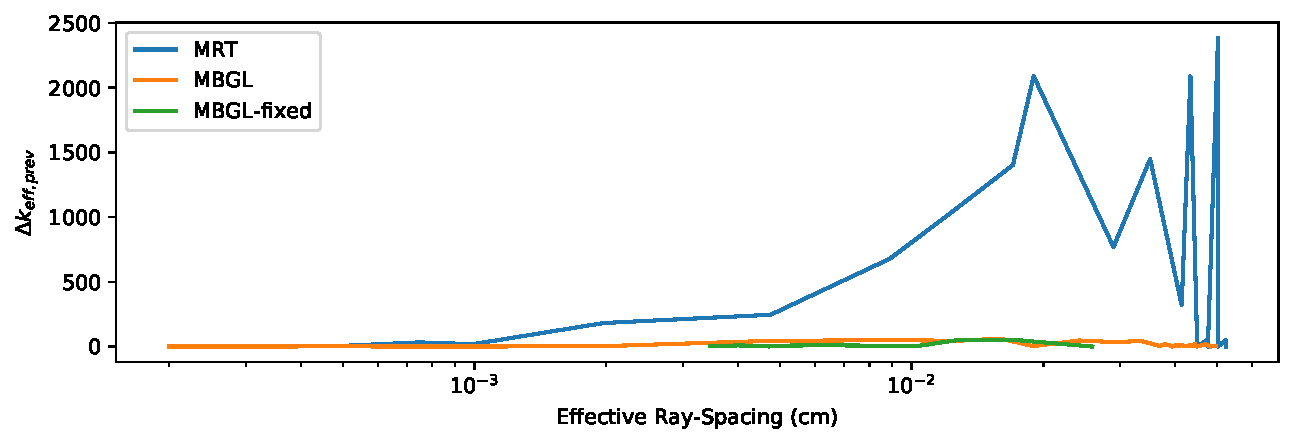
\includegraphics[width=0.95\linewidth]{\figpath/results/2D/1e/pdk-vs-rayspacing}
          \caption{VERA Problem 1E: Convergence of eigenvalue for different 2-D ray-tracing methods. \label{fig:MB:1e:pdk-vs-rayspacing}}
        \end{figure}
      }

      \subsubsection{VERA Problem 1E: 3-D}{\label{sssec:MR:1E:3-D}
        MPACT currently lacks a multigroup sweeper for 3-D self-shielding calculations, so this calculation was run without self-shielding.
        This will lead to a significantly different converged eigenvalue than for the 2-D case.
        However, even without self-shielding, this case can be used to show the benefits of the macroray ray-tracing method in 3-D \ac{MOC} calculations.
        Due to the 3-D rays, it is no longer useful to compare the results as a function of ray-spacing, as there is now the effective axial and effective radial ray-spacing.
        As it is a far better metric for the amount of work, all the 3-D results will simply use the number of track-segments for accuracy comparisons.
        Each calculation was run using od\ac{CMFD} acceleration \cite{Zhu2016}, and a directional quadrature with 64 azimuthal angles and 6 polar angles over $\fourpi$.

        \Cref{fig:MR:1e:3D:keff-vs-nSegs,fig:MR:1e:3D:pdf-vs-nSegs} show the $k$-eigenvalue as a function of the number of track segments, and the sequential differences in eigenvalue for each refinement of rays.
        These results compare the traditional \ac{MRT} method against the macroray method with a fixed number of rays in each radial and axial band (different amounts in radial and axial).
        A Gauss-Legendre quadrature was used to determine ray placement and width within each band.
        As this problem is axially homogeneous, a single ray was used in each axial band, and an axial ray-spacing of 0.75 cm was used for the \ac{MRT} method.

        These results suggest that the macroray method is able to converge toward the final result at a faster rate than the traditional \ac{MRT} method;
          the eigenvalue change between successive calculations (refining the number of rays) drops below 10 pcm with around 5.6 million segments, whereas the \ac{MRT} method was unable to converge within 10 pcm even using 14 million.
        Additionally, it is clear that the near-monotonic convergence behavior which the macroband had in 2-D holds in 3-D.

        The \ac{MRT} calculations were not continued past 14 million segments, as using finer ray-spacing resulted in significantly increased run-times, much of which was spent in the actual ray-tracing procedures.
        While the macroray does significantly simplify the ray-tracing procedure, the author believes that these long ray-tracing run-times in \ac{MRT} are likely due to unoptimized code, rather than an inherent flaw in the method.
        For 5.6 million segments, the macroray ray-tracing procedures took under 10 seconds, while for 4.8 million segments in the \ac{MRT} took 190 seconds.

        \begin{figure}[htbp]
          \centering
          \includegraphics[width=0.95\linewidth]{\figpath/results/3D/1e/keff-vs-nSegs}
          \caption{VERA Problem 1E: Eigenvalue results for different ray-tracing methods. \label{fig:MR:1e:3D:keff-vs-nSegs}}
        \end{figure}
        \begin{figure}[htbp]
          \centering
          \includegraphics[width=0.95\linewidth]{\figpath/results/3D/1e/pdk-vs-nSegs}
          \caption{VERA Problem 1E: Convergence of eigenvalue for different ray-tracing methods. \label{fig:MR:1e:3D:pdf-vs-nSegs}}
        \end{figure}
      }
    }

    \subsection{Shielded Fuel Box}{\label{ssec:MR:Shielded Fuel Box}
      The shielded fuel-box problem was created for this work to more clearly demonstrate the benefits of the macroray method for problems which pose challenges to the traditional ray-tracing methods.
      This problem consists of a 0.4$\times$0.4$\times$0.4 cm$^3$ fuel block surrounded on all sides by $0.1$ cm of a shielding material.
      This entire shielded cube is surrounded by 0.5$\times$0.5$\times$0.5 cm$^3$ cubes of moderator (26 in total).
      The calculation uses the C5G7 benchmark cross sections; the fuel is the 8.7\% \ac{MOX}, the shielding material uses the control rod cross sections.
      A 2-D cross-sectional view of the problem is shown in \cref{fig:MR:Shielded-Box Diagram}, and reflective boundary conditions are used on each face.
      This problem is meant to be similar to \ac{VERA} problem 1E, though the surrounding material was made thicker so that resolving the region did not require an extreme number of rays.

      The OpenMC Monte Carlo code \cite{OpenMC} was used to generate a reference eigenvalue to compare the results against.
      The reference solution was generated with 500 batches of 50000 particles, with 50 inactive batches.
      This yielded a reference eigenvalue with 4 pcm uncertainty.
      Each calculation used a Chebyshev-Chebyshev directional quadrature with 24 azimuthal and 12 polar angles over $\fourpi$;
        this quadrature was chosen, rather than a Chebyshev-Gauss, as the problem has the same axial and radial descriptions.
      Similarly, the radial and axial ray-spacing used by the \ac{MRT} are the same for each calculation, and the number of rays per radial or axial band are the same.

      \begin{figure}[h]
        \centering
        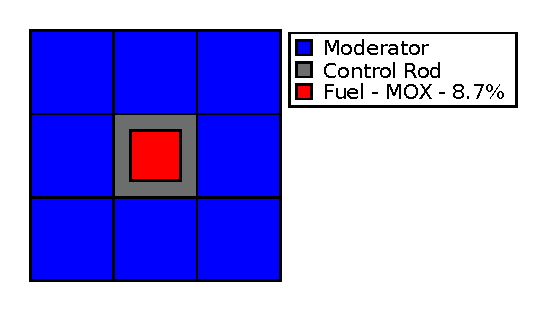
\includegraphics[width=0.75\linewidth]{\figpath/results/3D/shielded-box/ShieldedBox}
        \caption{Cross-sectional diagram of the shielded-box problem from x-y, x-z, or y-z directions. \label{fig:MR:Shielded-Box Diagram}}
      \end{figure}

      \begin{figure}[hp]
        \centering
        \includegraphics[width=0.95\linewidth]{\figpath/results/3D/shielded-box/keff-vs-nSegs}
        \caption{Shielded-Box Problem: Eigenvalue results for different 3-D ray-tracing methods. \label{fig:MR:SB:keff-vs-nSegs}}
      \end{figure}
      \begin{figure}[hp]
        \centering
        \includegraphics[width=0.95\linewidth]{\figpath/results/3D/shielded-box/dk-vs-nSegs}
        \caption{Shielded-Box Problem: Eigenvalue errors for different 3-D ray-tracing methods. \label{fig:MR:SB:dk-vs-nSegs}}
      \end{figure}
      \begin{figure}[hp]
        \centering
        \includegraphics[width=0.95\linewidth]{\figpath/results/3D/shielded-box/pdk-vs-nSegs}
        \caption{Shielded-Box Problem: Convergence of eigenvalue for different 3-D ray-tracing methods. \label{fig:MR:SB:pdk-vs-nSegs}}
      \end{figure}

      The results of the ray-tracing methods are summarized in \cref{fig:MR:SB:keff-vs-nSegs,fig:MR:SB:dk-vs-nSegs}.
      The traditional \ac{MRT} method is able to generate very large eigenvalue errors when a coarse ray-spacing is used;
        in fact, for the first several ray-spacing values used, the eigenvalue estimate was near critical even though the reference is very sub-critical.
      This shows a major flaw in the \ac{MRT} methods, they don't consider the internal geometry and allow for such coarse spacings that the results can be entirely useless.
      In contrast, the macroray method enforces a minimum number of rays which seems to give somewhat reasonable results.

      \Cref{fig:MR:SB:pdk-vs-nSegs} shows the change in eigenvalue for each sequential calculation (a refinement in the number of rays/segments).
      This figure shows that for the very coarse ray-spacings, that resulted in a near critical eigenvalue, don't have very large differences.
      An inexperienced user may believe that the solution is near convergence, which is certainly not the case.
      Once the ray-spacing is smaller than the thickness of the shielding the results become reasonable, although still further off from the reference than the macroray method for the same number of segments.
      However, a user without knowledge of the \ac{MOC} would likely not be aware that this is a requirement of the user input.
      Although this was demonstrated with very coarse ray-spacings, a similar effect would likely be present if the shielding were thinner than the default ray-spacing of MPACT.
      This shows a clear advantage for the macroray method, in that it allows the user to use the method without detailed knowledge of the method.
    }

    \subsection{C5G7}{\label{ssec:MR:C5G7}
      % The C5G7 [CITATION] benchmark was the primary benchmark case used to evaluate the initial capability of the macroray ray-tracing method.
      % The benchmark is commonly used as part of the verification of neutronics codes, both 2-D and 3-D.

      The C5G7 \cite{Smith2002,Smith2006} benchmarks are a set of benchmark problems commonly used to help the verification of 2-D and 3-D transport methods.
      The original benchmark specified a 3-D problem, and a second benchmark reduced the axial size of this problem and added configurations with inserted control rods.
      In this work, each of the three extended 3-D benchmark problems are solved using both the traditional ray-tracing method (\ac{MRT}), and the new macroray ray-tracing method.
      \cref{figs:MR:C5G7:Layout} shows the configuration of the C5G7 core benchmark cases; the different problems differ only in their axial description.
      The radial layout of each fuel assembly is shown in \cref{fig:MR:C5G7:RadialAssemblyLayout}.

      The \ac{LSA} was used for all of the calculations in this work, and the meshing parameters used were found to be sufficient in previous studies on the \ac{LSA} [CITATION].
      In the axial direction, the problem was meshed into 2.38 cm slices.
      The rods (fuel, guide-tubes, and control rods), used a single radius of 0.540 cm, with 4 azimuthal divisions, and 8 azimuthal divisions in the surrounding moderator.
      The reflector pins used a radial mesh of 0.42$\times$0.42 cm$^2$.
      A Chebyshev-Gauss directional quadrature with 64 azimuthal angles and 8 polar angles over $\fourpi$ was used, as it was shown to yield good agreement in previous works with 3-D \ac{MOC} \cite{Kochunas2013}.
      A pin-wise modular ray-tracing was used, with each ray-tracing module being 1.26$\times$1.26$\times$2.38 cm$^3$.

      \begin{figure}[htbp]
        \centering
        \begin{subfigure}[t]{0.45\textwidth}
          \centering
          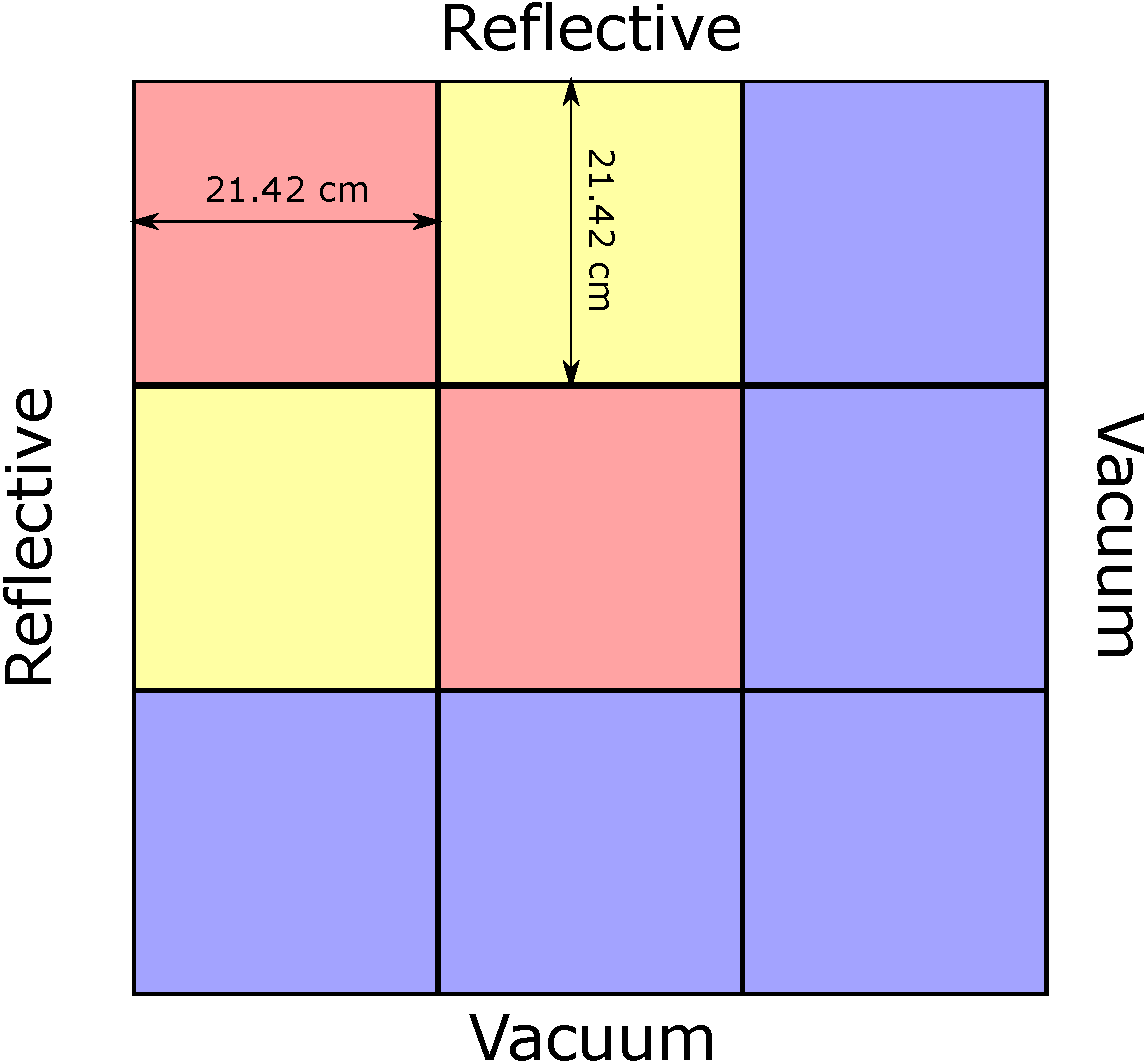
\includegraphics[width=0.9\textwidth]{\figpath/results/3D/C5G7/Diagrams/C5G7-RadialLayout}
          % \caption{\label{fig:MR:C5G7:RadialLayout}}
        \end{subfigure}%
        ~
        \begin{subfigure}[t]{0.45\textwidth}
          \centering
          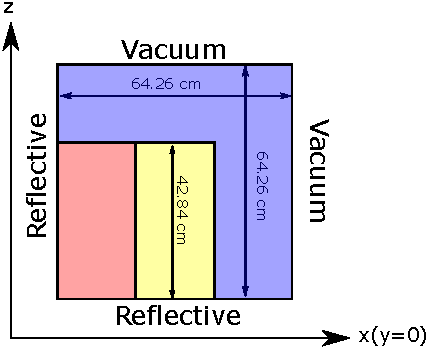
\includegraphics[width=0.9\textwidth]{\figpath/results/3D/C5G7/Diagrams/C5G7-AxialLayout}
          % \caption{fig-2\label{fig:fig-2}}
        \end{subfigure}
        \begin{subfigure}[t]{0.65\textwidth}
          \centering
          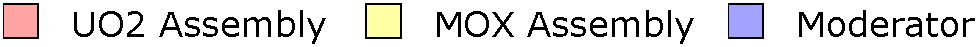
\includegraphics[width=0.9\textwidth]{\figpath/results/3D/C5G7/Diagrams/C5G7-Legend}
          % \caption{fig-2\label{fig:fig-2}}
        \end{subfigure}
        \caption{C5G7 extended benchmark core layouts. \label{figs:MR:C5G7:Layout}}
      \end{figure}

      \begin{figure}[htbp]
        \centering
        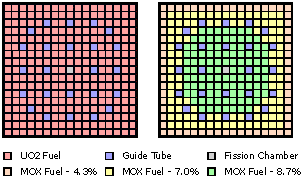
\includegraphics[width=0.85\linewidth]{\figpath/results/3D/C5G7/Diagrams/C5G7-RadialAssemblies}
        \caption{C5G7 Assembly layouts.\label{fig:MR:C5G7:RadialAssemblyLayout}}
      \end{figure}


      % \subsubsection{C5G7 Pin-Cells}{\label{sssec:MR:C5G7:Pin-Cells}

      % }

      % \subsubsection{C5G7 Mini-Case}{\label{sssec:MR:C5G7:Mini-Case}

      % }

      \subsubsection{C5G7 Benchmark: Unrodded}{\label{sssec:MR:C5G7:Unrodded}
        The unrodded case has no control rods inserted into the fuel, but control rods are present in the axial reflector region above the fuel region.
        This is shown in \cref{fig:MR:C5G7:Unrodded}.

        \begin{figure}[htbp]
          \centering
          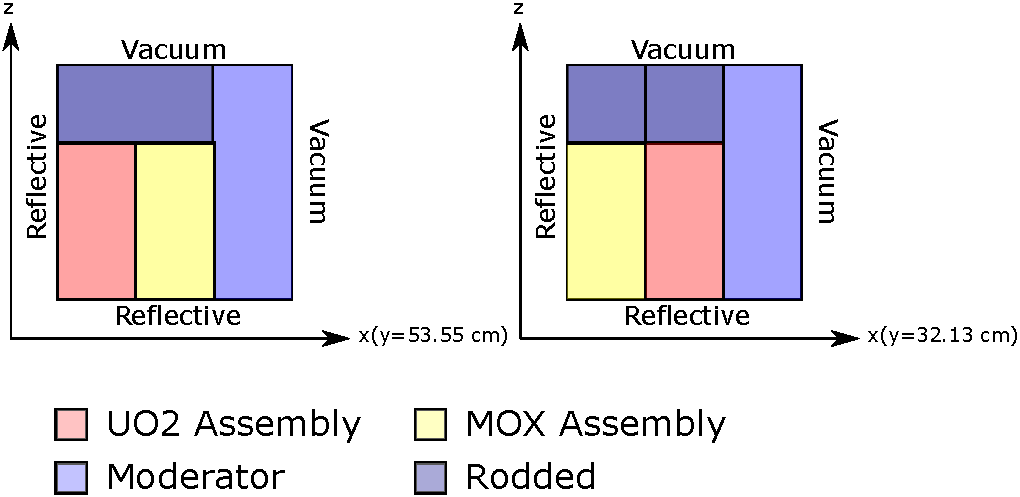
\includegraphics[width=0.85\linewidth]{\figpath/results/3D/C5G7/Diagrams/C5G7-Unrodded}
          \caption{C5G7 Benchmark: Unrodded core configuration. \label{fig:MR:C5G7:Unrodded}}
        \end{figure}
      }

      \subsubsection{C5G7 Benchmark: Rodded A}{\label{sssec:MR:C5G7:Rodded A}
        The C5G7 rodded A case has control rods partially inserted 14.28 cm, one third of the fuel height, into the central \ac{UO2} assembly.
        The remaining \ac{UO2} assembly and \ac{MOX} assemblies have no inserted control rods.
        The core layout is depicted in \cref{fig:MR:C5G7:Rodded A}.
        \begin{figure}[htbp]
          \centering
          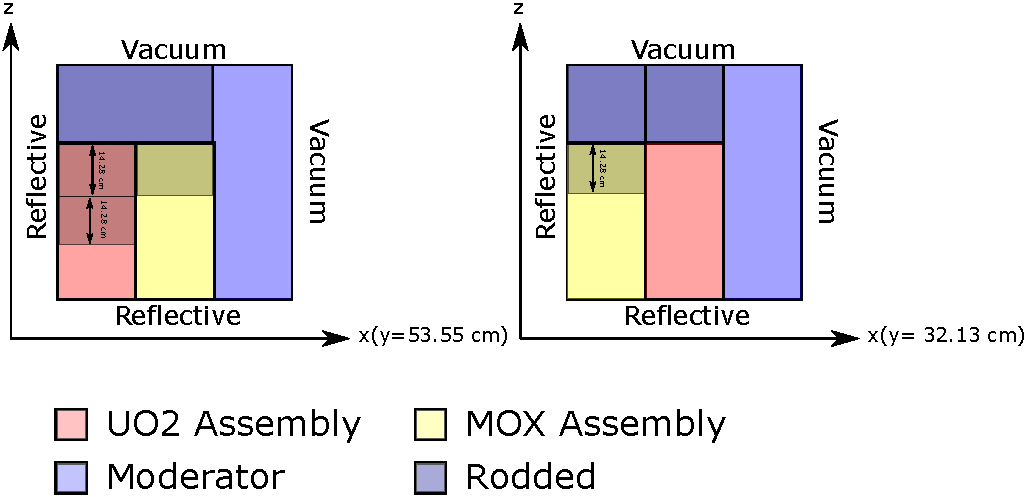
\includegraphics[width=0.85\linewidth]{\figpath/results/3D/C5G7/Diagrams/C5G7-RoddedB}
          \caption{C5G7 Benchmark: Rodded A core configuration. \label{fig:MR:C5G7:Rodded A}}
        \end{figure}
      }

      \subsubsection{C5G7 Benchmark: Rodded B}{\label{sssec:MR:C5G7:Rodded B}
        The C5G7 rodded B case has control rods partially inserted into three of the four fuel assemblies.
        Each of the \ac{MOX} assemblies has control rods inserted 14.28 cm.
        The center \ac{UO2} assembly has control rods inserted 28.56 cm, two thirds of the fuel height; the outer \ac{UO2} assembly has no inserted control rods.
        This layout is depicted in \cref{fig:MR:C5G7:Rodded B}.

        \begin{figure}[htbp]
          \centering
          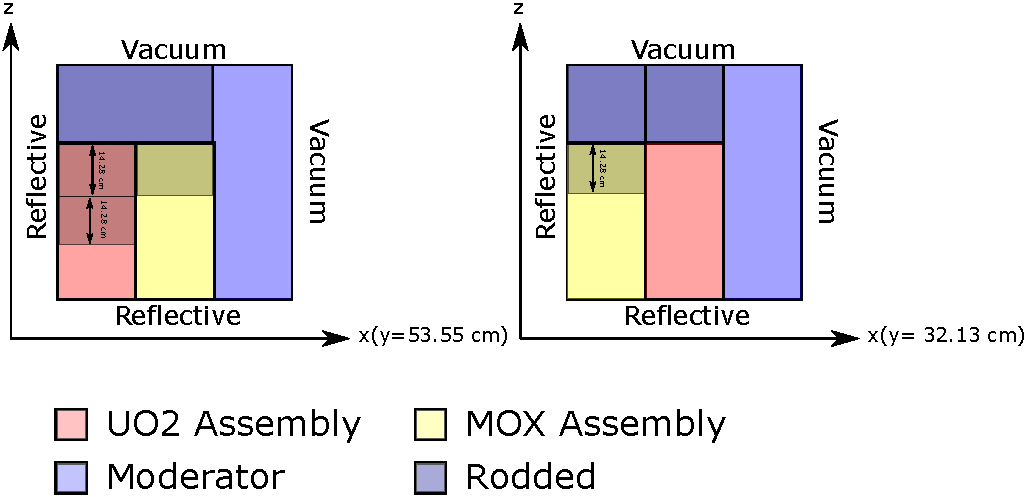
\includegraphics[width=0.85\linewidth]{\figpath/results/3D/C5G7/Diagrams/C5G7-RoddedB}
          \caption{C5G7 Benchmark: Rodded B core configuration. \label{fig:MR:C5G7:Rodded B}}
        \end{figure}
      }
    }
  }

  \section{Conclusions}{\label{sec:MR:Conclusions}

  }
  % References
  \printbibliography
}